\section{System Architecture}
%	* high order feature: arc heat change, influence of 2 order feature, feature template
%	* learning: MIRA, converge of training
%	* pseudocode of mapper(avoid circle) framework
%\KZ{Rephrase the following. What do you mean by attach? Also try not to be too casual, e.g., think about...}
%\BF{Mcdonald's example graph of decoding: ROOT John saw a dog yesterday which was a Yorkshire Terrier.}
In the following, we present the preliminary investigation on the two key
components of the our parser: head mapper and sequence predictor .
%\KZ{This should go into discussions after presenting the approach: Since we only try out limited number of possible approaches,
%more work could be embedded in this framework to
%replace either component, which may lead to closer results to the upper bound we give out in the experiment.}

\subsection{Head Mapper}
%We first give an example to explain how head mapper actually works. Then we explain
%the features and scorer embeded in the head mapper. Finally, we describe the method to train the scorer model.
\begin{figure*}[th]
\centering
\epsfig{file=exampleparse_emnlp.eps, width=0.9\columnwidth}
\caption{Example Parse of head mapper}
%for the sentence ``\emph{John saw a dog yesterday which was a Yorkshire Terrier}". Red node is the child to be processed in every step; red arc is the final attachment from head to its dependent and dashed arc is left out to avoid circle in the parse tree.}
\label{fig:egparse}
\end{figure*}

%\KZ{The first letter of some words are missing in the figure.}
\figref{fig:egparse} shows the decoding process of the head mapper
for a non-projective example sentence~\cite{mcdonald2005non}:
``\emph{John saw a dog yesterday which was a Yorkshire Terrier}".
%\KZ{What's the original sentence? Present it first.}
%\KZ{You don't have to repeat the CoNNL format. It's not important.}
%Pseudocode shows how the head mapper works.
%Our decoder works just as the process in \figref{fig:egparse}.
%\BF{pseudocode of head mapper decoding and symbol explainations here}
A head mapper takes the lexical information of a sentence and
a permutated sequence of words in that sentence as inputs.
Suppose the sequence is: % from MaltParser:

\noindent
$John_{1}\rightarrow a_{3}\rightarrow dog_{4}\rightarrow yesterday_{5}\rightarrow Yorkshire_{9}\rightarrow a_{8}\rightarrow was_{7}\rightarrow which_{6}\rightarrow Terrier_{10}\rightarrow saw_{2}.$

The subscript stands for the position of the word in original sentence.
At step one, we look for the head of \textit{John}. At this point,
all other words are potential candidate heads. In order to measure
the probabilities of these candidate arcs, we introduce a scorer, which
is the key idea of graph-based parsers. By comparing the scores
printed on every black arc in \figref{fig:egparse},
the red arc was eventually selected, i.e. $saw$ is made the head
of $John$. The process continues for the word \textit{a}, etc.

In practice, we
%maintain a disjoint set of words processed to
ensure that
there are no cycles of nodes generated during parsing, so that the final output
is a dependency tree structure starting from
the ROOT node\footnote{A manually introduced node in dependency parsing task,
it is the root of a dependency tree.}.
We also build a parse agenda to record the existing arcs, which
provides the high order information for our scorer.
%\KZ{More details here?
%What does the parse agenda look like? How does it support high order parsing?
%Maybe use the example?}
For example, after adding arc:$saw \rightarrow John$ , all
the attachment on these two nodes will take this arc into consideration.
%For a sentence with $N$ words, the final result consists of
%($N+1$) nodes and $N$ arcs.
%\KZ{You don't need to remind people over and over again this is a combination of
%MST and Malt. You just say what you did, if it's something that MST and Malt have
%done before, be very brief about this part, and give a citation. This paper
%is about your work, not about MST or Malt.}
%Both MaltParser and MSTParser treat projective and non-projective dependency tree discriminatively. MaltParser define an extra action SWAP to generate projectivization transformation of a non-projective dependency tree \cite{nivre2009non}.
%There is a drawback of MaltParser that it cannot generate non-projective output providing projective training set, because there are no SWAP action in oracle transitions. It is sensible to look into the relation between
%possible word pairs directly. But word order limits the word pairs considered in MaltParser. MSTParser employ Chu-Liu-Edmonds algorithm to decode non-projective cases \cite{mcdonald2005non}
%and Eisner algorithm to deal with projective trees\cite{mcdonald2005online}. Though Chu-Liu-Edmonds algorithm is a solution to unify projective and non-projective cases, it declines the accuracy while applying on projective trees. Our decoder also unifies these two situations and
%searches heads globally. It directly measures the relative closeness between every possible head and current processing word and generate non-projective tree naturally.
%Head mapper tries to map head for every word stepwise according to a given process sequence of words.
%\KZ{It makes sense to include an example here to illustrate the head-mapper.}
%\subsection{Scorer and features}
%In order to simulate this process,

We introduce a linear arc scorer to measure the score of a directed arc.
The sum of all arc scores gives the final score of the whole parse tree.
%\BF{formula of arc score model}
%\[
%\text{Score}(\mathbf{y})=\displaystyle{\sum_{(i,j)\in\mathbf{y}}} \mathbf{w} \cdot \mathbf{f}(i,j)
%\]
%In this formula, $i,j$ are the indexes of an arc in parse tree $\mathbf{y}$. The inner product of arc feature vector $\mathbf{f}(i,j)$ and weight vector $\mathbf{w}$ represents score of an arc $(i,j)$. By summing up all the
%arc scores, we can get final score of the whole parse tree $\mathbf{y}$.
We currently use the typical high-dimensional binary features,
%\BF{feature template table}
including second order features \cite{mcdonald2006online}.
%\KZ{Maybe
%name some of the major features here. Don't expect the readers to
%read the MST paper.}
%As the previous statement, feature scope in graph-based parser
%is limited by decoding algorithm and several works successfully
%adapt Eisner algorithm to include high order features .
Because of the deterministic decoding in our framework,
we can make use of existing arcs to guide later head mapping.
This kind of decoder gives us the flexibility of applying any
high order features explored by previous
works~\cite{carreras2007experiments,koo2010efficient,ma2012fourth}.
%\KZ{For example?}
%\KZ{Again, you are making it sound like you only did some minor changes to MST.
%This is not the right style to write about your work. You can say we use a modified
%verion of MIRA~\cite{}, in which we did blah..}
%Based on different decoding and factoring methods, graph-based models employ different learning algorithms to induce the feature weights. Among them, variant perceptron algorithms are widely used \cite{kubler2009dependency}.

The arc scorer is trained by the iterative online
training framework MIRA (Margin Infused Relaxed Algorithm)~\cite{crammer2003ultraconservative}.
%\KZ{Give citation of MIRA itself instead of citing MST.}
\cut{
The updating constraint is defined as
\begin{align*}
&\text{min}\|\mathbf{w}^{(i+1)}-\mathbf{w}^{(i)}\|\\
&\text{s.t. } s(\boldsymbol{x}_t,\boldsymbol{y}_t)-
s(\boldsymbol{x}_t,\boldsymbol{y}')\ge L(\boldsymbol{y}_t,\boldsymbol{y}')
%\\&\forall \boldsymbol{y}'\in \text{dt}(\boldsymbol{x}_t)
\end{align*}
where $\mathbf{w}^{(i)}$ are the feature weights for the $i$-th iteration,
$\mathbf{x}_t$ and $\mathbf{y}_t$ are sentence and its gold parse tree,
respectively. $\mathbf{y}'$ is the output of our parser with $\mathbf{w}^{(i)}$ and
score margin is given out by a loss function $L$.
}
%On each update, MIRA attempts to keep the norm of the change to the parameter vector as small as possible, subject to
%correctly classifying the instance under consideration with a margin at least as large as the loss of the incorrect classifications \cite{mcdonald2005online}.
%\BF{this is the original sentence in this paper}
%Similarly, we define the loss function as the number of incorrect arcs to apply MIRA to dependency parsing and it
%is represented as following formula: \BF{Is this formula necessary ?}
%\BF{MIRA formula}
%\KZ{Don't like the following sentence.}
%From this definition, the only change we should make is replacing the exact inference decoder with our deterministic
%decoder.
In each iteration, we update the feature weights based on one sentence. The
decoder gives a greedy parse according to current feature weights.
By scoring the gold dependency tree and the current parse,
along with the number of incorrect arcs in the current parse,
MIRA keeps updating the weights until it eventually converges to an optimal scorer.
The learning algorithm typically terminates after a few iterations.
%(\figref{fig:itertest}).
%\BF{Converge graph of head mapper}
%\begin{figure}[htp]
%\centering
%\epsfig{file=itertest.eps, width=\columnwidth}
%\caption{Accuracy curves on training set. \newline Test on first 100 sentence of WSJ senction 00.}
%\label{fig:itertest}
%\end{figure}

\subsection{Sequence Predictor}
%A sequence predictor either selects the word to process stepwise, or generates an complete word sequence.
\cut{
We developed three different sequence predictors. The first two are based on
offline training (one is a learning to rank algorithm and the other is
an action classifier used in MaltParser) from ``gold'' parsing sequences,
and produce a complete parsing sequence given a sentence.
The third sequence predictor is unsupervised and is
integrated with the decoding process, i.e. it produces the next word to
process based on the current parsing configuration.
Next we briefly discuss these three approaches.
}
%We state the rule of gold sequence in Section 2 and we can generate gold sequences with the gold dependency trees.
%Sequence predictor then learns from these gold sequences and tries to produce a sequence
%for new sentences.
%
%\subsection{Effects of Sequences}
%\KZ{Not sure what ``Sequence dependence'' means. Headings should be self-explanatory
%and clean. Consider rephrase the following paragraph. Very garbbled.}
%As we point out in section 2, getting a gold sequence from a gold dependency tree is not a one-to-one mapping.
%\BF{breadth-first traversal and malt convert sequences of example sentence}
%For example, there is a breadth-first traversal sequence of the sentence in \figref{fig:egparse},
%$which_{6}\rightarrow was_{7}\rightarrow a_{8}\rightarrow Yorkshire_{9}\rightarrow a_{3}\rightarrow Terrier_{10}\rightarrow John_{1}\rightarrow dog_{4}\rightarrow yesterday_{5}\rightarrow saw_{2}$
%, which is also a gold sequence along with the example sequence.
%\subsection{Pairwise learning to rank}
\cut{In this approach, we attempted two ways to generate gold parsing sequences.
First is a bottom-up, breadth-first traversal of the gold parse tree. This
way we are essentially processing words which are lower down in the parse
tree first, which are often less important modifiers, before moving to words
which are more central to the syntactic structure of the sentence.
The second is to take the training data from a converting function of
MaltParser, which converts a gold parse tree into a sequence of actions.
We can infer the parsing sequence of words from the sequence of actions.}

%We human beings execute a few pairwise comparisons to decide the next
%word to be processed, which is similar to preference learning problem in learning to rank.
%Sequence predicting is also a ranking process. We select next word to process by comparing it with the other words in a pairwise way.
%Viewing the task of sequence predictor in this way,
%preference learning problem in learning to rank gives a solution to predict.
\cut{
\textbf{Pairwise learning to rank }We can decompose a gold sequence into pairwise partial orders between
two words and train a binary classifer to determine the order of any two
words within a sentence. This is a popular approach in learning to rank.
However, combining pairwise orders into a complete sequence is an NP
problem~\cite{grotschel1984cutting},
we therefore use a greedy algorithm
from Schapire et al.~\shortcite{schapire1998learning} to produce such a sequence.
}
%\subsection{Action classifier in MaltParser}
The intuition of sequence predictor
is to rank words according to the ease of head word attaching.
Words that are easy to handle can be processed earlier without high order features.
To decide whether process a word immediately, we imitate the action classifier in MaltParser.
\cut{
MaltParser employs a
classifier to determine what parsing action (e.g.,
{\em shift}, {\em push}, etc.) to take at each step. The whole parsing
process defines a sequence of such actions. Although this sequence is
not exactly the word sequence used in our system, such a word sequence
can be inferred rather straightforwardly from the action sequence.

Another advantage of
the MaltParser is that it's extremely fast. Therefore, we can use MaltParser
to quickly parse through a given sentence, record the action sequence and
infer the parse sequence from it.
}
%
%Inspired by our left-to-right analysis of a sentence, we either find
%head for current word or skip this hard word and scan on. This is obviously a classification problem and
%MaltParser happen to hold the same view.\BF{cannot say so now} MaltParser add arc incrementally and provide us a potential sequence.

In fact, we can understand the action classifier in a different way that it can reflect the relative
priority between the top two words on processing stack. We translate the actiones as:
\begin{itemize}
\setlength{\itemsep}{0pt}
\setlength{\parsep}{0pt}
\setlength{\parskip}{0pt}
 \item LA - process the word on the top of stack;
 \item RA - process the second word in stack;
 \item SH - postpone the process of both the two words on top of stack.
\end{itemize}
In this way, a word sequence
can be inferred rather straightforwardly from the action sequence.

%We can decompose the predicting process into two steps:
%getting pairwise rank of every two nodes and aggregating
%these partial results into a complete process sequence.
%
%We apply LIBLINEAR\footnote{\urlstyle{same}\url{http://www.csie.ntu.edu.tw/~cjlin/liblinear/}} to training a binary classifier to get the priority of every two words. The training data are pairwise orders extracted from the gold sequence.
%The classifier can then be used to predict the relative ordering for any two words with a confidence score.
%\BF{Jia fill the details: rankSVM, Cohen, citation of preference learning}

%  \item {\bf Malt} The oracle sequence generated by converting function in MaltParser.
%  \item {\bf Random} A random permutation sequence of words for a sentence.
%  \item {\bf Increase} The left-to-right sequence, which means we process the sentence with
%  the word index increasing.
%\end{itemize}
%
%In order to test how the sequence quality influence decoding and measure different types of sequences,
%we generate four types of sequence files to test on the head mapper.
%%The train set is transformed by StanfordParser on WSJ section 2-21 and test set on WSJ section 00-01.
%Types of sequences are list below:
%Among them, the Malt sequence outperforms other types of the sequences.
%In the following, we describe a few alternative approaches to predict the sequences.
%%        \item[1] The breadth-first traversal sequence of a sentence
%        \item[2] The oracle sequence generated by converting function in MaltParser.
%        \item[3] Predicting process sequence of MaltParser stackproj algorithm.
%        \item[4] The random permutation sequence of words in a sentence.
%        \item[5] The left to right sequence, word indexes are process sequences.
%{\bf Breadth-first} The breadth-first traversal sequence of a sentence.
%
%{\bf MaltConvert} The oracle sequence generated by converting function in MaltParser.
%
%{\bf MaltPredict} Predicting process sequence of MaltParser stackproj algorithm.
%
%{\bf Random} The random permutation sequence of words in a sentence.
%
%{\bf Increase} The left to right sequence, word indexes are process sequences.
%{\small
%~\\
%
%$\bullet$ Oracle {\bf converting} sequences of MaltParser.
%
%$\bullet$ {\bf Breadth-first} traversal of a gold parse tree.
%
%$\bullet$ {\bf Predicting} process sequence of MaltParser.
%
%$\bullet$ A {\bf random} words permutation of the sentence.
%
%$\bullet$ A word sequence with {\bf increasing} index from left to right of the sentence.
%\begin{table*}[htbp]
%  \centering
%  \caption{Cross test of sequence type}
%  %\begin{threeparttable}
%    \begin{tabular}{Il|cccccIccI}
%    \whline
%    %\diagbox{Test}{Train}& Breadth-first\tnote{1} & MaltConvert\tnote{2} & MaltPredict\tnote{3} & Random\tnote{4} & Increase\tnote{5} & Average & StdDev \\
%    \diagbox{Test}{Train}& MaltConvert & Breadth-first & MaltPredict & Random & Increase & Average & StdDev \\
%    \hline
%    MaltConvert & 93.59\% & 67.32\%  & 93.29\% & 89.50\% & 83.91\% & 85.52\% & 0.109 \\
%    Breadth-first & 79.65\% & 92.36\% & 80.93\% & 86.46\% & 84.75\% & 84.83\% & 0.050 \\
%    MaltPredict & 89.30\% & 66.07\%  & 89.50\% & 87.14\% & 82.36\% & 82.87\% & 0.098 \\
%    Random & 55.41\% & 48.84\% & 56.49\% & 70.92\% & 62.77\% & 58.89\% & 0.083 \\
%    Increase & 48.89\% & 46.98\% & 48.83\% & 65.18\% & 63.36\% & 54.65\% & 0.088 \\[2pt]
%    \whline
%    \hline
%    %\midrule[3pt]
%    %     &       &       &       &       &       &     &  \\
%    Average & 73.37\% & 64.31\% & 73.81\% & 79.84\% & 75.43\%      &     & \\
%    StdDev & 0.201 & 0.183 & 0.200 & 0.110 & 0.113     &     & \\
%    \Cline{1.5pt}{1-8}
%    \end{tabular}%
%    %\begin{tablenotes}
%%        \footnotesize
%%        \item[1] The breadth-first traversal sequence of a sentence
%%        \item[2] The oracle sequence generated by converting function in MaltParser.
%%        \item[3] Predicting process sequence of MaltParser stackproj algorithm.
%%        \item[4] The random permutation sequence of words in a sentence.
%%        \item[5] The left to right sequence, word indexes are process sequences.
%%      \end{tablenotes}
%%\end{threeparttable}
%  \label{tab:crosstest}%
%\end{table*}%
%\subsection{Attempts}

%\subsection{Feature score based predictor}
%{\bf Scorer-based  }
\cut{
The intuition of sequence predictor
is to rank words according to the ease of head word attaching.
Words that are easy to handle can be processed earlier without high order features.
\cut{Words that are processed later are harder and may require high order
features. }
Since the head mapper can score every possible arc,
for each word $w$, we can compute a list of scores for all the candidate
head word of $w$. If there is a large difference in scores between the best
candidate head word and the remaining candidates for $w$,
then we can conclude the processing $w$ doesn't require high order features
and therefore can be done early.
}
%High order features are available later in the parsing process
%because many arcs have been attached by then.
%this score naturally reflects the possibility that
%a certain word can be the head of another word. We consider a word to be
%easy to deal with if
%A word is easy to deal with means that there is a head candidate much more possible than other candidates, so that it is no need to employ higher order features to find a head. In other words, greater the difference is, harder can higher order features make up for the difference.
%The intuition of sequence predictor is ranking words according to the ease
%of head word attaching. Now that the head mapper can score all possible
%head words and then choose the one with highest score, this score
%can be seen as the confidence of this arc. An arc with higher confidence
%is naturally easier to deal with.
%A word is easy to deal with means that there is a head candidate gets a higher score than the other candidates.
\cut{
As such, we maintain a matrix $M_{(n+1) \times n}$ to store the scores of
head-dependent pairs, which are initially calculated by the first order
features. When a new arc is added to the parse tree, we remove the
cells that may form a cycle with the existing arcs and update the cells
relating to this new arc using higher order features.}
%Each time we choose the word with greatest difference between its highest score and second highest score.
%After we build an arc,
 %and update sibling scores (different high order structures may require more updates).

%We will compare these three approaches in some preliminary evaluations next.
%~\\
%}
%\BF{table of cross test}

%The result of this cross test is in \tabref{tab:crosstest}. As we can
%see, training result relies much on the sequence information. Breadth-first sequence
%and MaltConvert sequence are both gold sequence of a sentence. These gold sequence models
%cannot obtain the best accuracy in other types of test sequence. Instead, the accuracy is determined
%by two factors. One is the quality of sequence, the other is matching degree between train
%sequence type and test sequence type. We can also tell from this table that we can get a
%high accuracy with a good type of sequence even on our greedy head mapper.
%
%The average accuracy and standard variance for sequence type of train file indicates the
%ability to match other types of sequence. Better sequence type gets a higher
%standard variance and a lower average accuracy. Random sequence approaches to all types in
%some sub-sequences. Increase sequence approaches to the two gold sequence because their nodes
%in the same level on gold trees mainly follow a left-to-right process rule.
%
%However, the average accuracy and standard variance for sequence type of test file shows
%the quality of a sequence type. Worse types of sequence struggles in parameter updates
%in training and better types test file can obtain a not bad result on models of worse types.
%On the contrary, worse types get bad performance on models of better types. So the accuracy
%of test file is limited by the quality of sequence type.
%%\BF{interesting conclusions: in Report201516doc, good order+ greedy head mapper->good result}
%
%Further, we print out the first-order arc heat map of same sentence.
%\BF{arc heat map}
%As we can see, different models score the arcs quite differently. Scorer relies much on the sequence and
%matched sequence pattern in train set and test set promise a high accuracy, which makes sequence predictor
%an interesting but hard task.
